\section*{Problem Statement}
The objective of this problem is to approximate the amplitude decay of a \textbf{damped harmonic oscillator} using rational interpolation. Given discrete amplitude measurements over time, the goal is to reconstruct the amplitude curve, evaluate it at specific time points, and visualize the interpolation.

\begin{quote}
  \textbf{NOTE}: The code can be accessed using this link: \href{https://raw.githubusercontent.com/HavokSahil/computational-techniques-assignments/refs/heads/main/assignment5/a2.m}{MATLAB}, \href{https://raw.githubusercontent.com/HavokSahil/computational-techniques-assignments/refs/heads/main/assignment5/a2.jl}{Julia}.
\end{quote}

\section*{Methodology}
The amplitude of a damped harmonic oscillator decreases over time. Given a set of discrete samples of amplitude versus time:
\[
(T_i, A_i) = \{(0, 10), (2, 5.5), (4, 3.5), (6, 2.6)\},
\]
we reconstruct a continuous approximation using \textbf{rational interpolation}.

\subsection*{Rational Interpolation}
1. \textbf{Reciprocal Difference Table:}
   - Construct the difference table \(D\) using a reciprocal-based scheme:
   \[
   D[i,1] = A_i, \quad D[i,j] = \frac{T_{i+j-1} - T_{j-1}}{D[i+1,j-1] - D[1,j-1]}.
   \]
2. \textbf{Rational Interpolant Construction:}
   - Using the extracted coefficients \(A\) from \(D\), the rational interpolant is recursively defined as:
   \[
   R(t) = A_1 + \frac{t - T_1}{A_2 + \frac{t - T_2}{\dots + \frac{t - T_{N-1}}{A_N}}}.
   \]

\subsection*{Steps}
\begin{enumerate}
    \item Construct the reciprocal difference table from the given amplitude samples.
    \item Extract rational coefficients for interpolation.
    \item Evaluate the interpolant over a fine time grid \(0:0.1:6.0\) s.
    \item Compute the amplitude at \(t = 5.0\) s as an example.
    \item Plot the interpolated curve along with the original data points for visualization.
\end{enumerate}

\section*{Results}
- The rational interpolant reconstructs the amplitude decay smoothly over the entire time interval.
- At \(t = 5.0\) s, the interpolated amplitude is:
\[
A(5.0 \text{ s}) \approx 2.9550
\]
- The plot shows that the interpolated curve passes closely through all measured data points, maintaining the expected decay behavior.

\begin{figure}[h!]
  \centering
  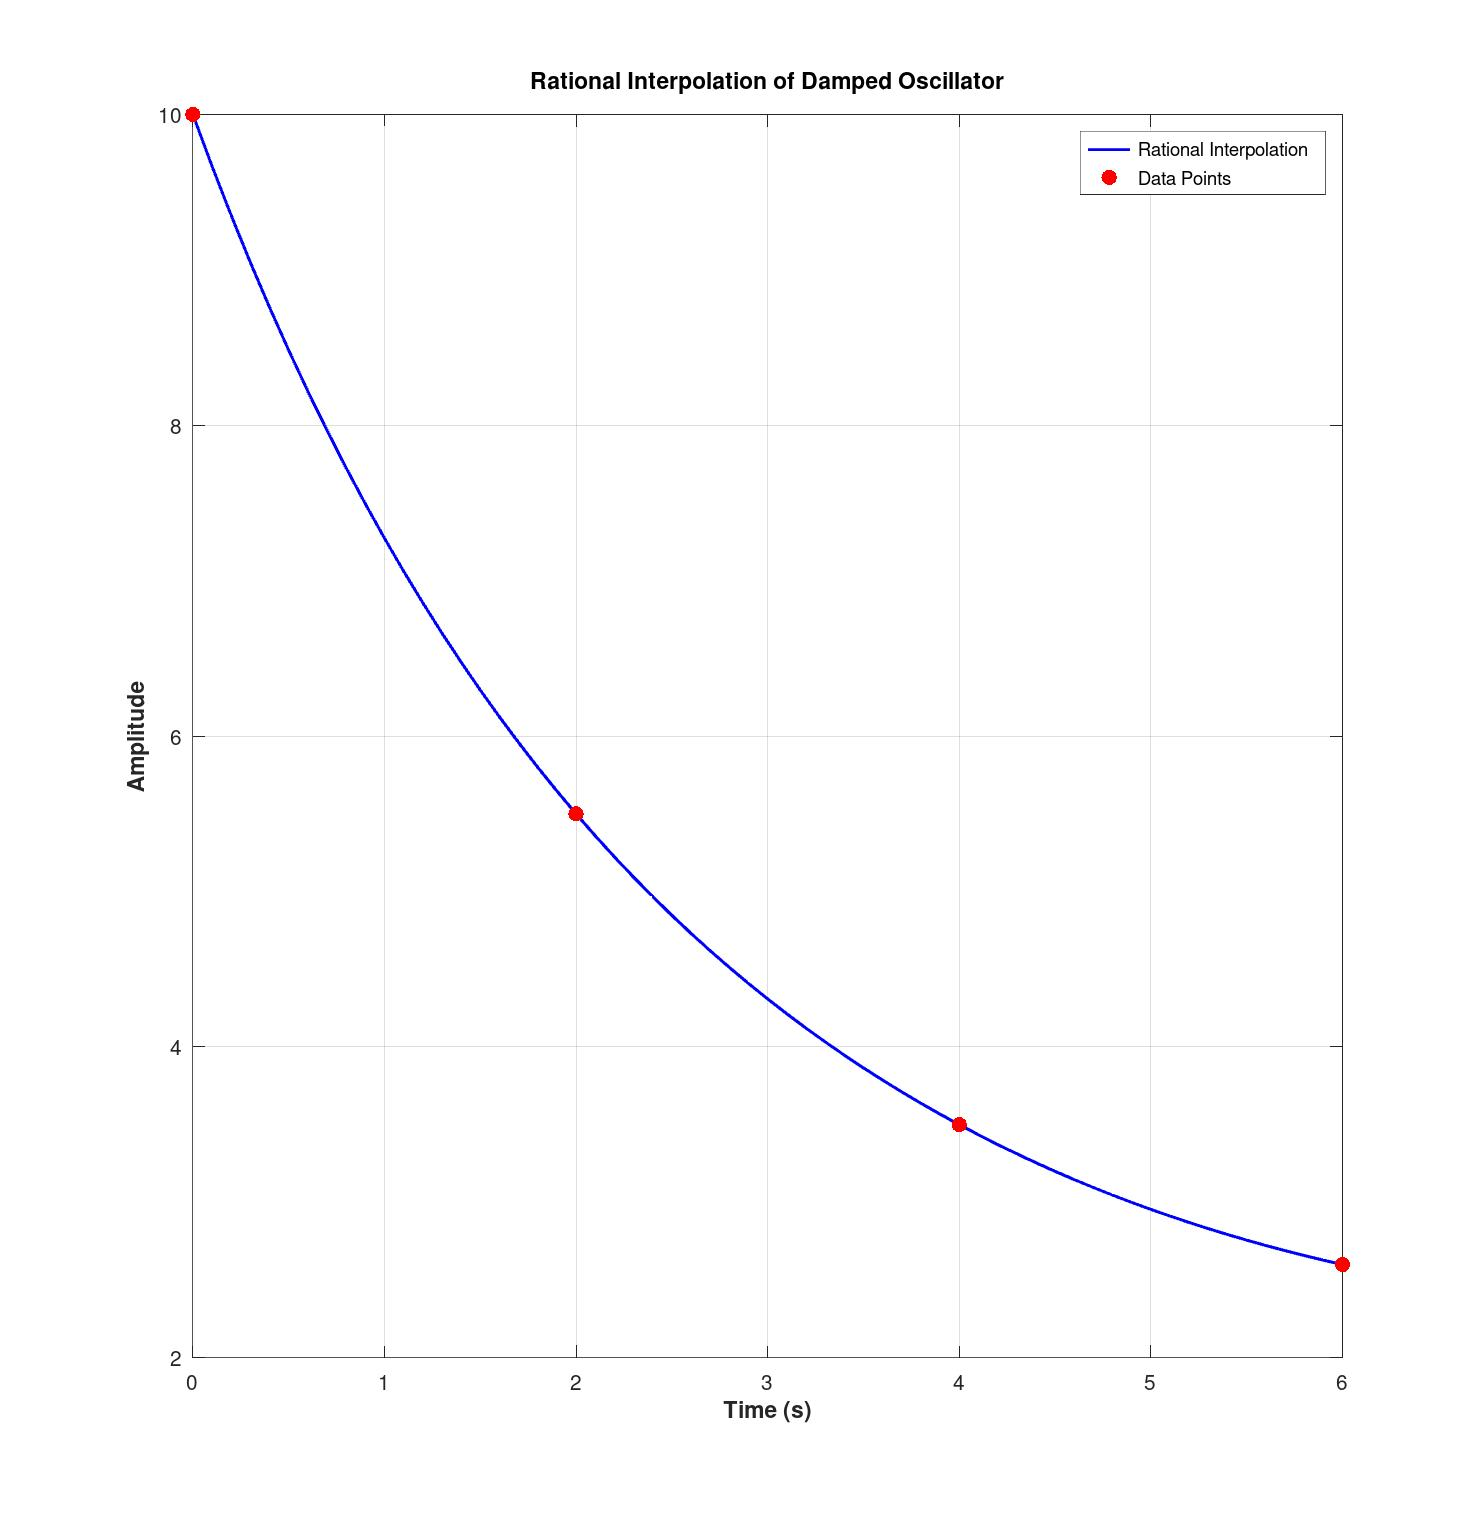
\includegraphics[width=0.93\textwidth]{a2.jpg}
  \caption{Rational interpolation of the damped harmonic oscillator amplitude (blue line) and original data points (red circles).}
\end{figure}

\section*{Conclusion}
Rational interpolation successfully reconstructs the amplitude decay curve from discrete measurements of a damped harmonic oscillator. The interpolated values match the trend of the original data, providing a smooth approximation and enabling estimation at intermediate time points. This demonstrates that rational interpolation is effective for modeling decaying or rapidly changing signals where polynomial interpolation might produce oscillations or inaccuracies.
